\section{Qt?} 

\begin{frame}
  \frametitle{Qt?}
  \begin{itemize}
  \item A C++ framework for Desktop and Mobile apps\pause
  \item Abstracting "platforms": \\
    (stdlib, {\bf windowing system}, {\bf GUI}, VFS, networking, "XML", \ldots)\pause
  \item Cross-platform: \\
    Linux (X11, Wayland, Android), macOS, iOS, Windows, Blackberry, Sailfish OS, \ldots
  \end{itemize}
\end{frame}

\begin{frame}
  \frametitle{Used by KDE}
  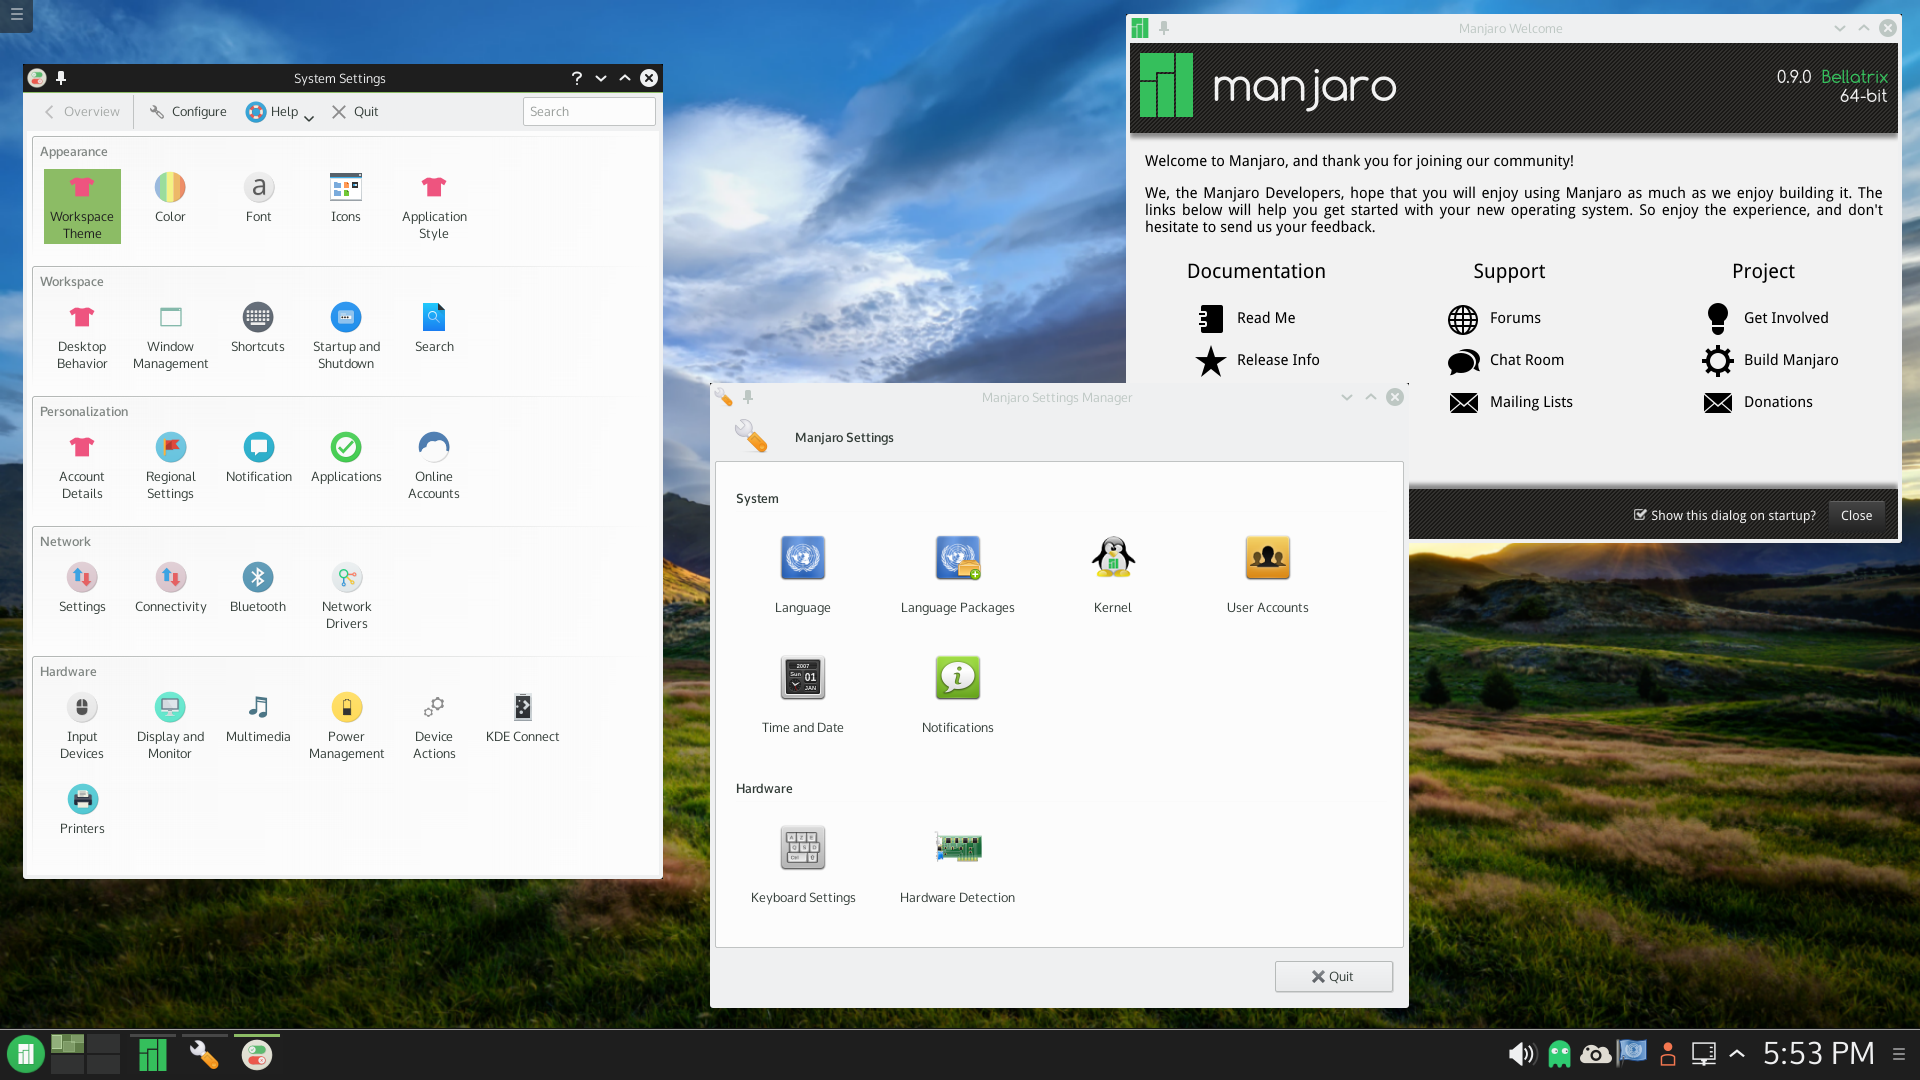
\includegraphics[width=\textwidth]{apps_kde}
\end{frame}

\begin{frame}
  \frametitle{Google Earth}
  %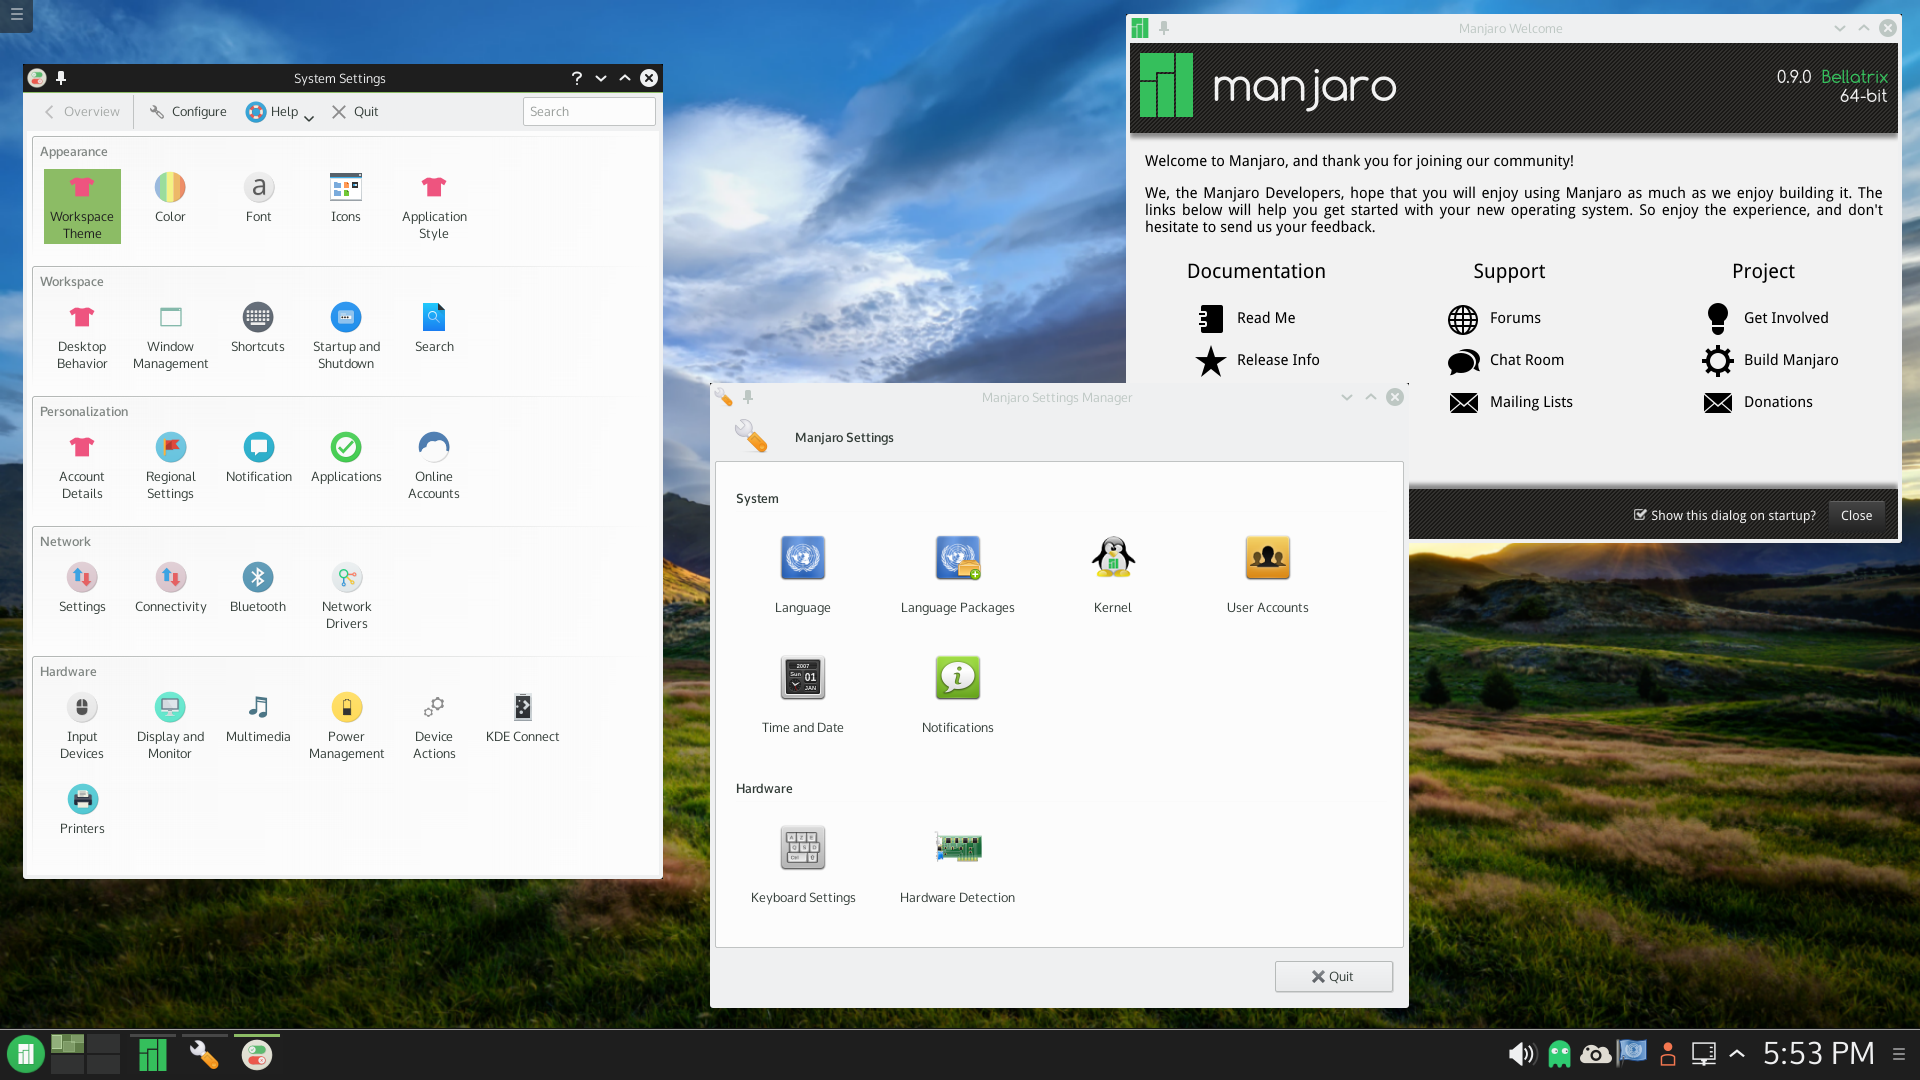
\includegraphics[height=\textheight,width=\textwidth]{apps_kde}
  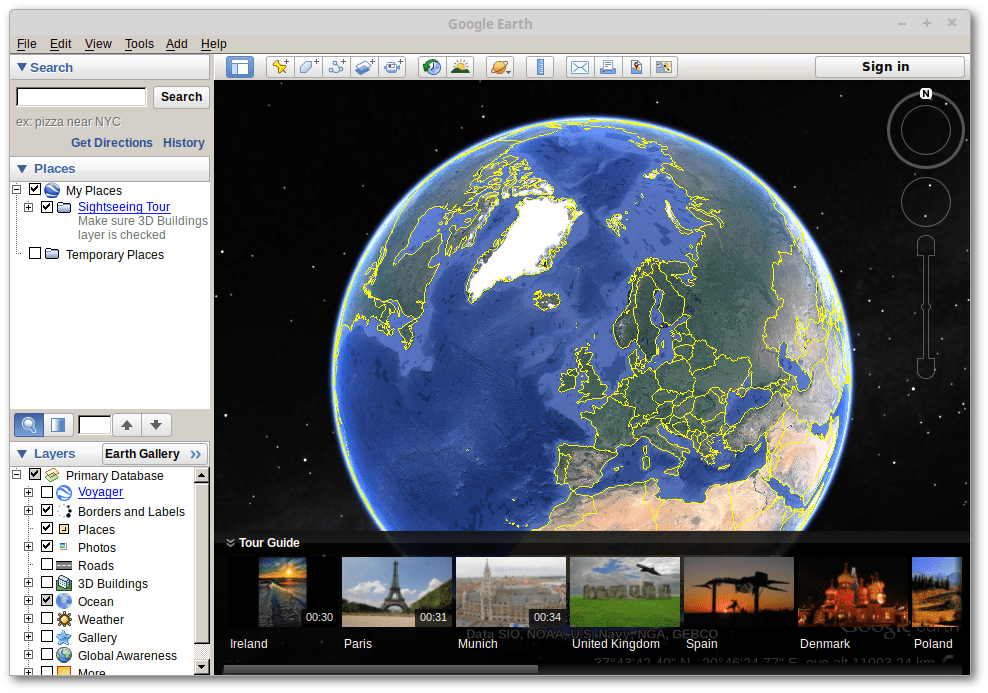
\includegraphics[height=0.9\textheight]{apps_earth}
\end{frame}

\begin{frame}
  \frametitle{Adobe Photoshop Elements}
  %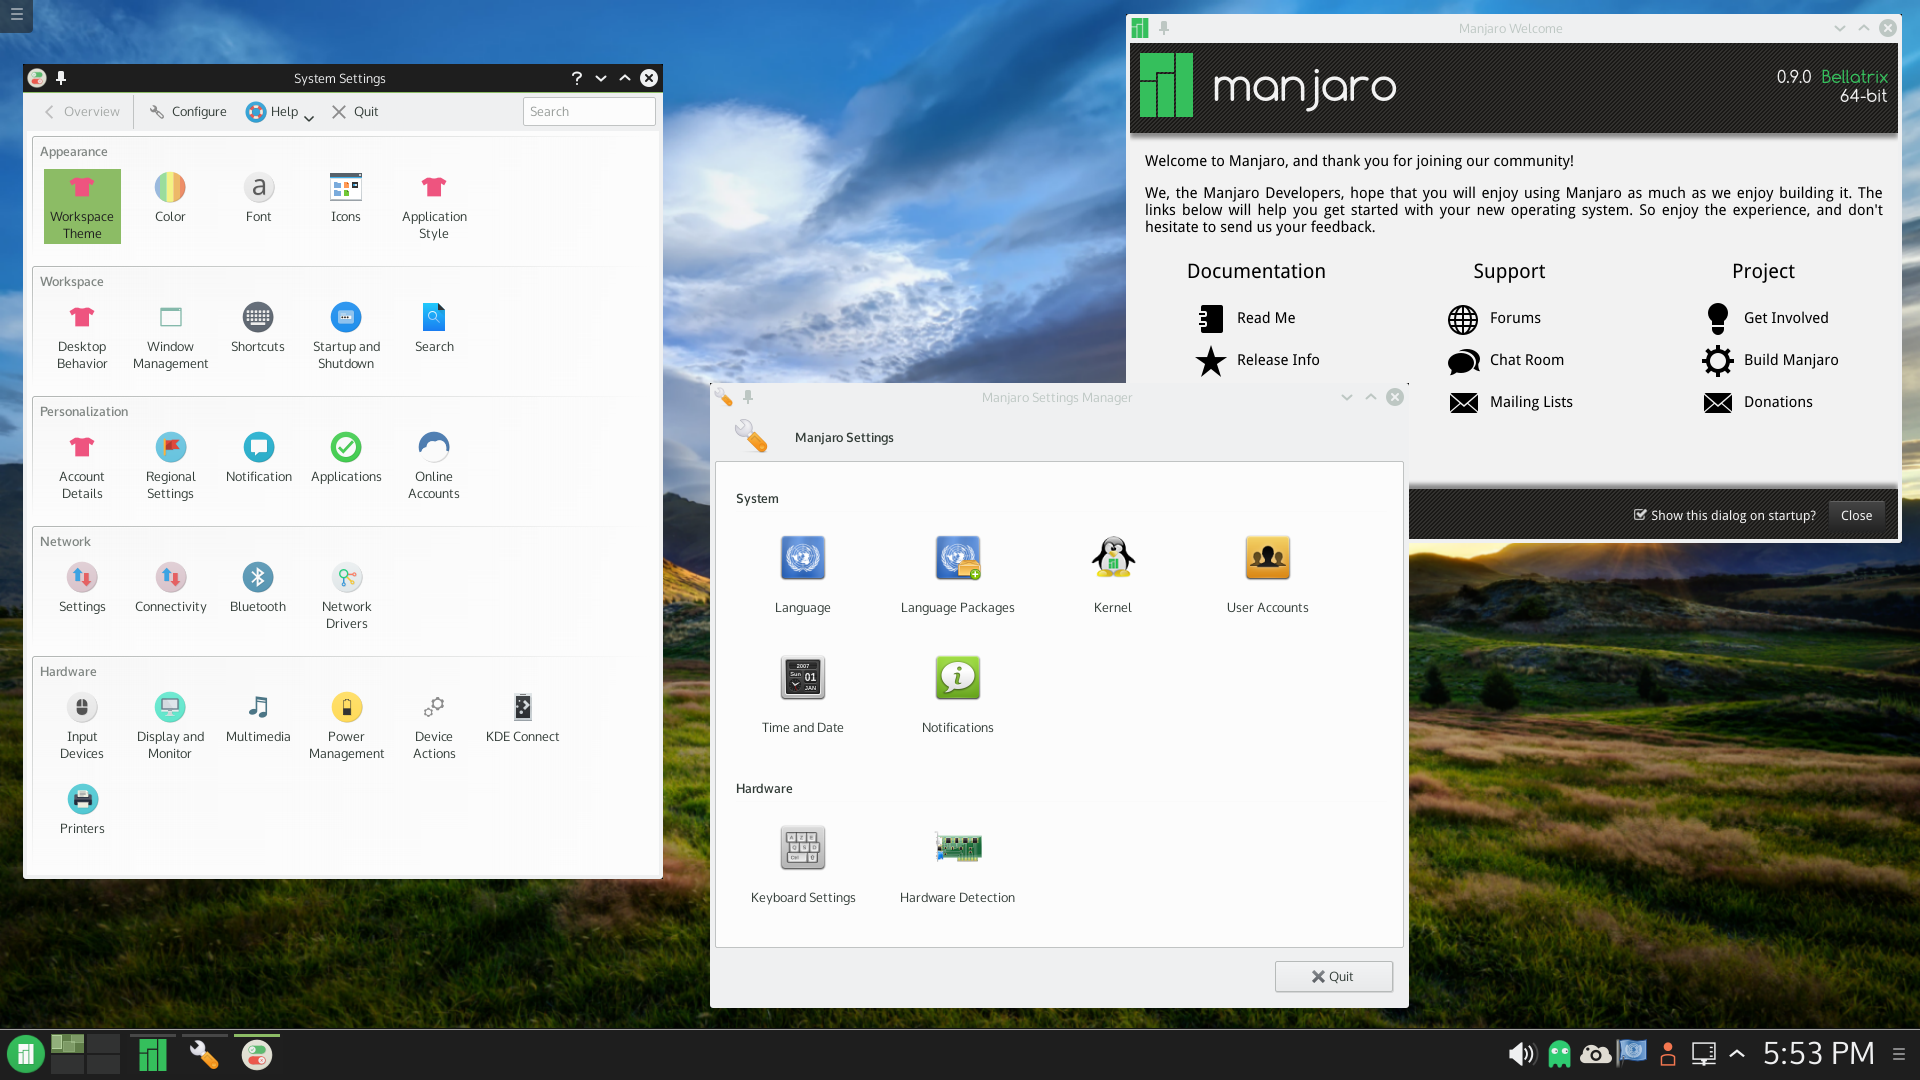
\includegraphics[height=\textheight,width=\textwidth]{apps_kde}
  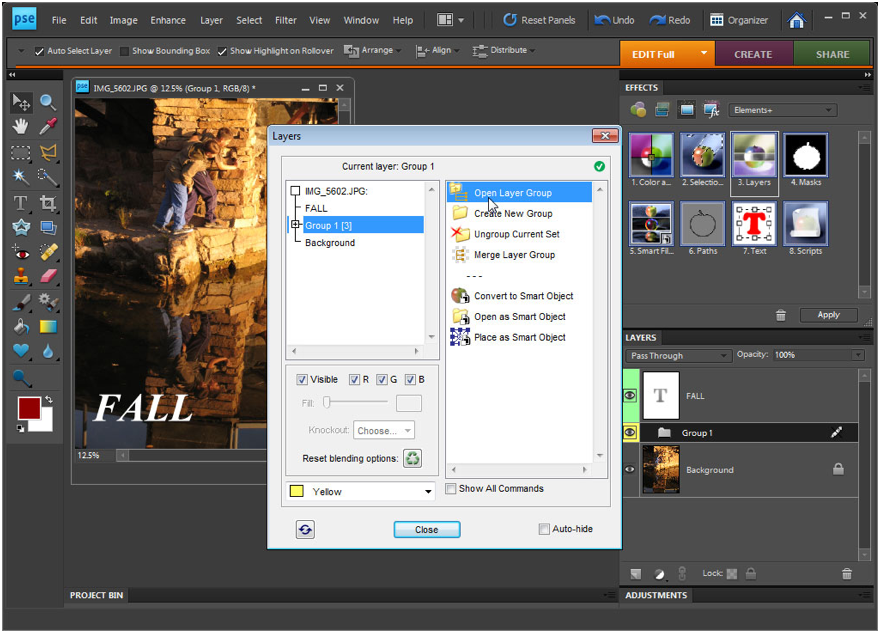
\includegraphics[width=\textwidth]{apps_photoshop}
\end{frame}

\begin{frame}
  \frametitle{AMD Code XL}
  %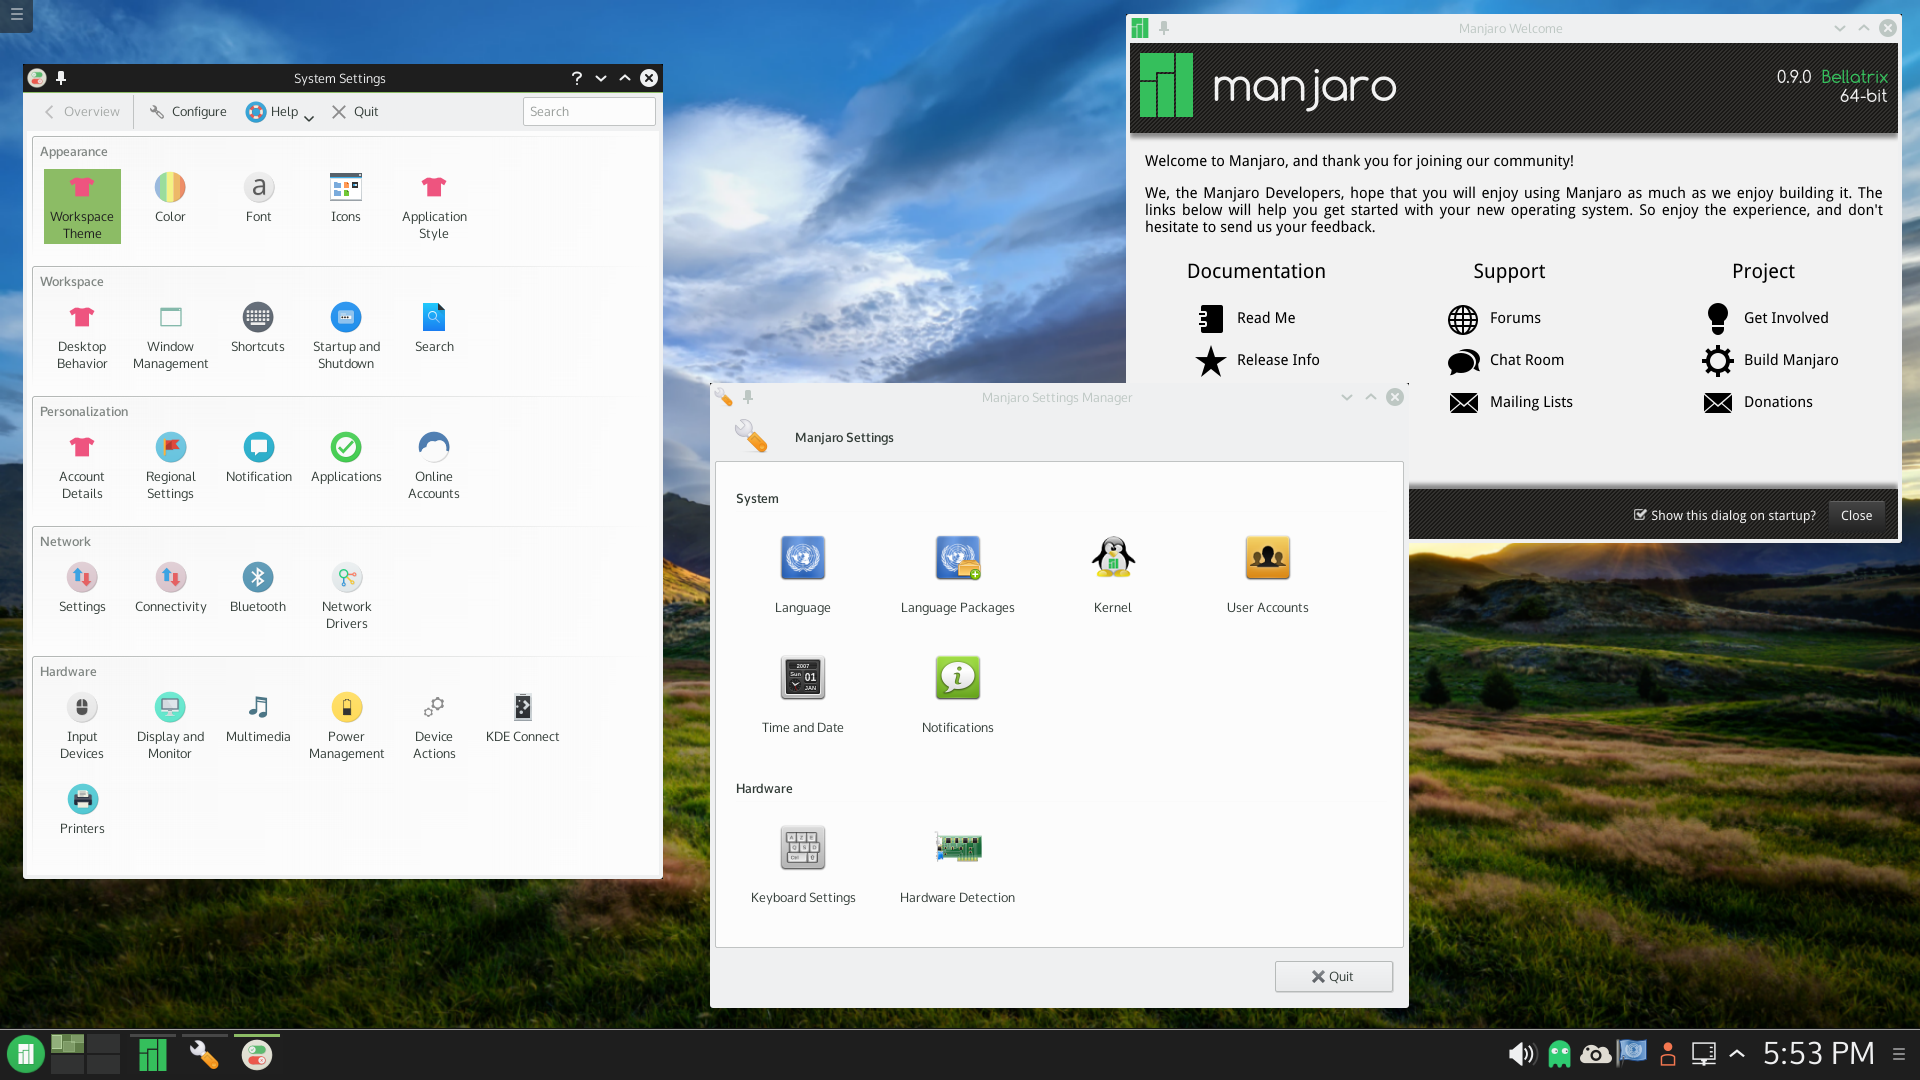
\includegraphics[height=\textheight,width=\textwidth]{apps_kde}
  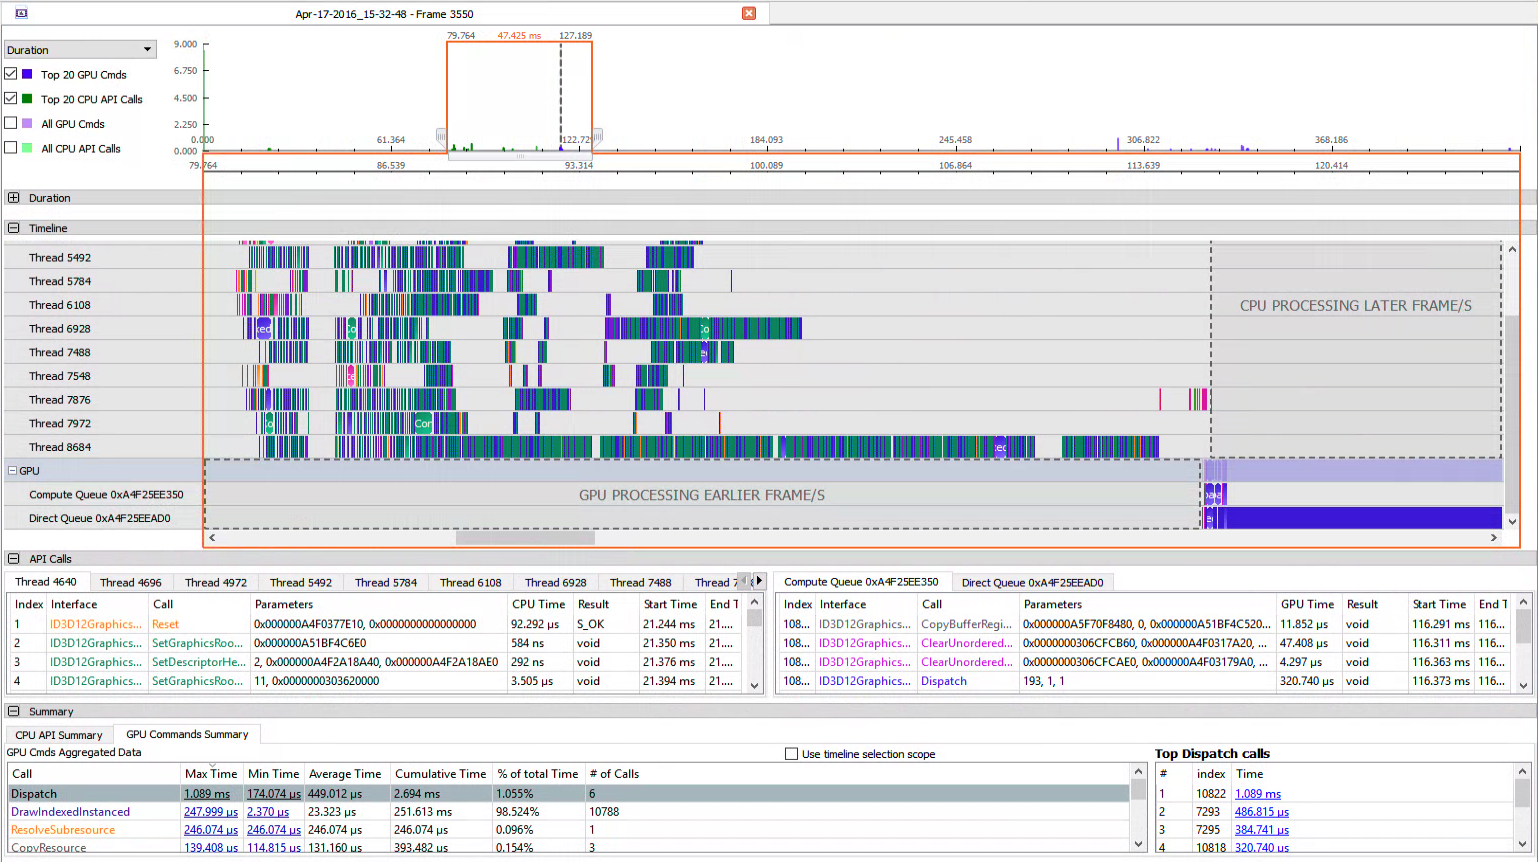
\includegraphics[width=\textwidth]{apps_codexl}
\end{frame}

\begin{frame}
  \frametitle{Musescore (Desktop)}
  %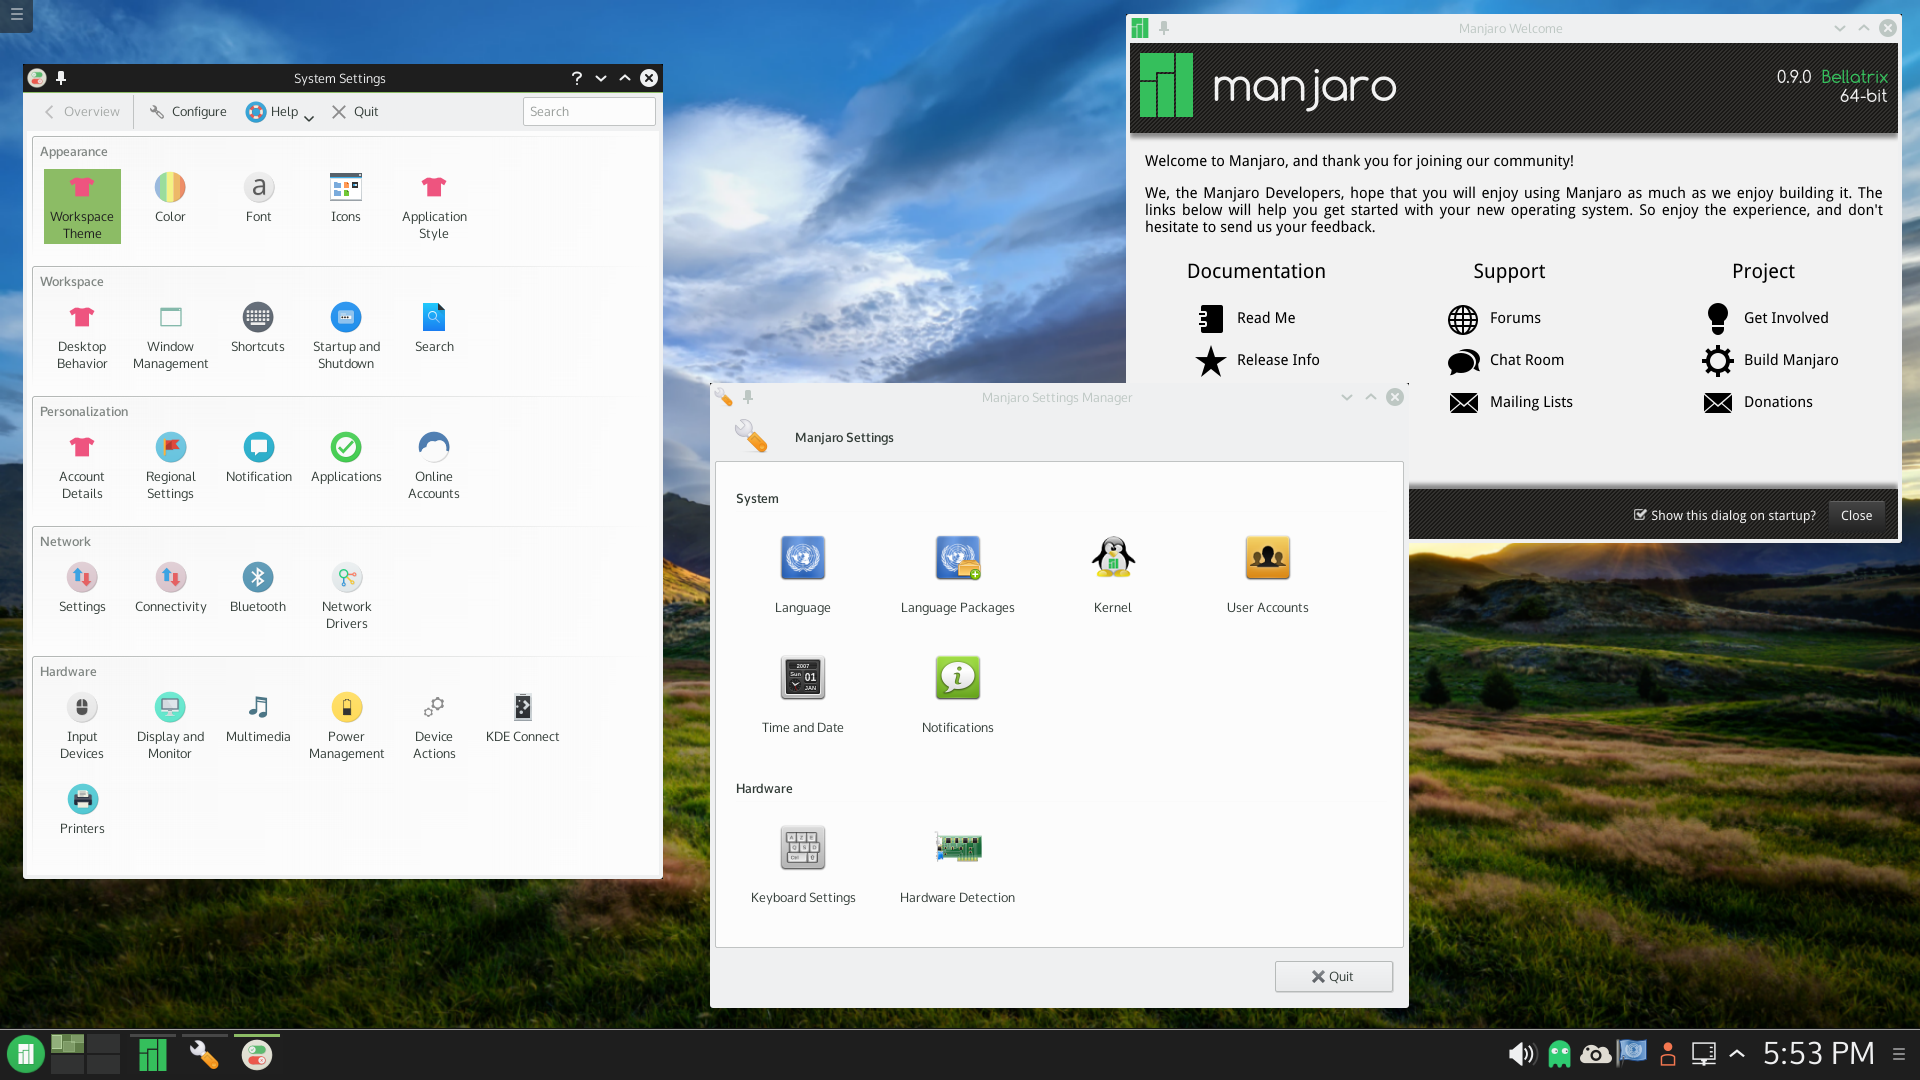
\includegraphics[height=\textheight,width=\textwidth]{apps_kde}
  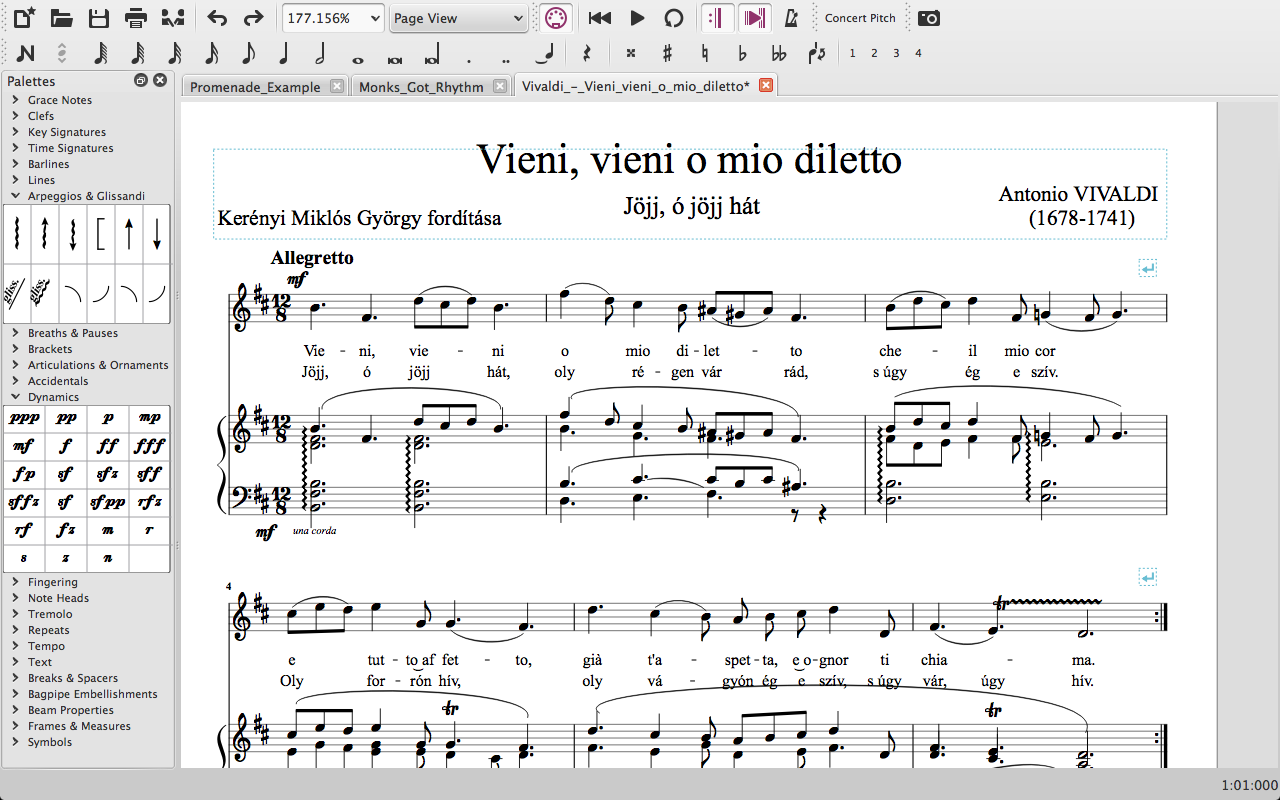
\includegraphics[width=\textwidth]{apps_musescore}
\end{frame}

\begin{frame}
  \frametitle{Musescore (iOS)}
  \center
  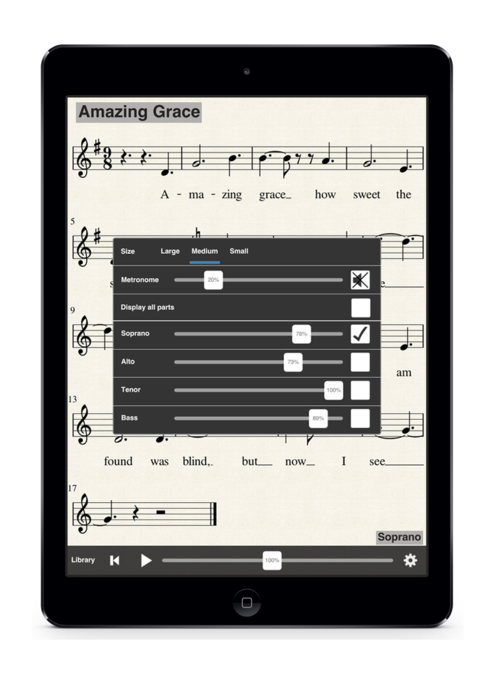
\includegraphics[height=0.9\textheight]{apps_musescore_ios}
\end{frame}

\begin{frame}
  \frametitle{Musescore (Android)}
  %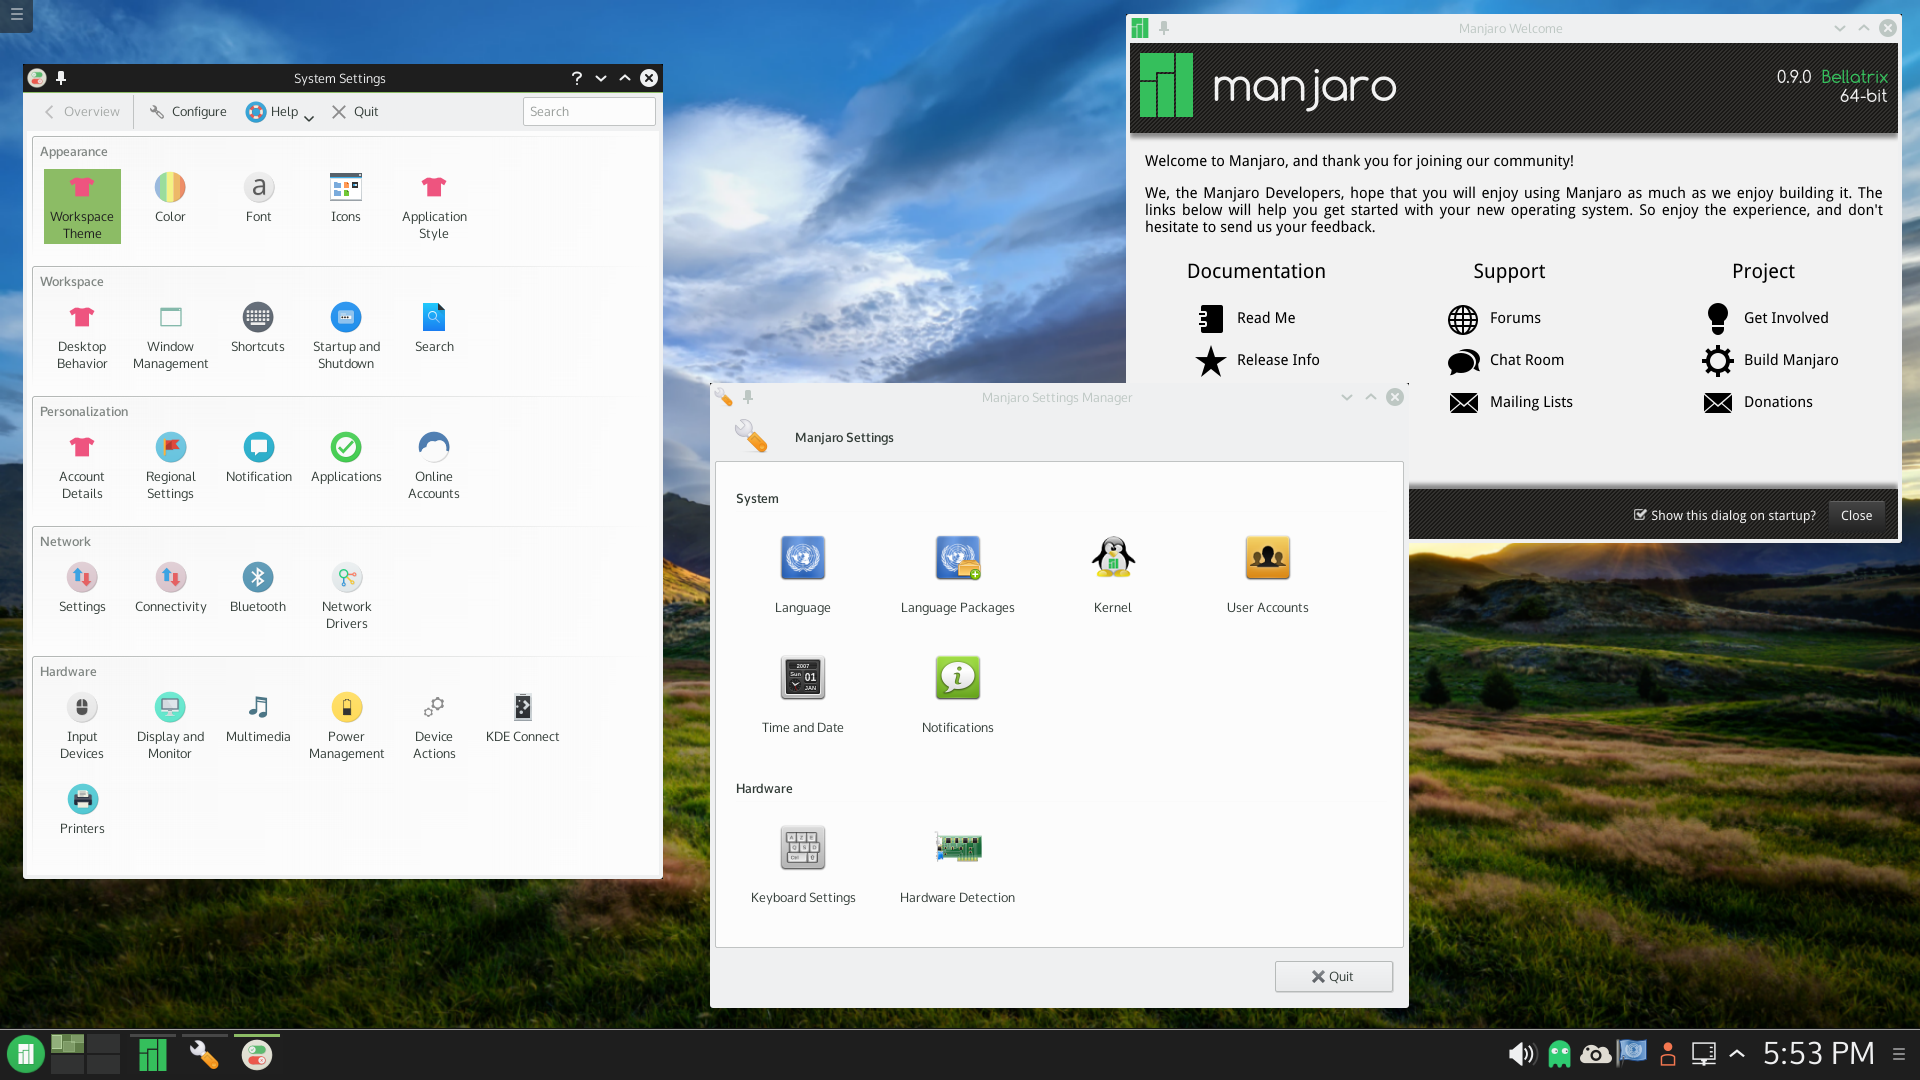
\includegraphics[height=\textheight,width=\textwidth]{apps_kde}
  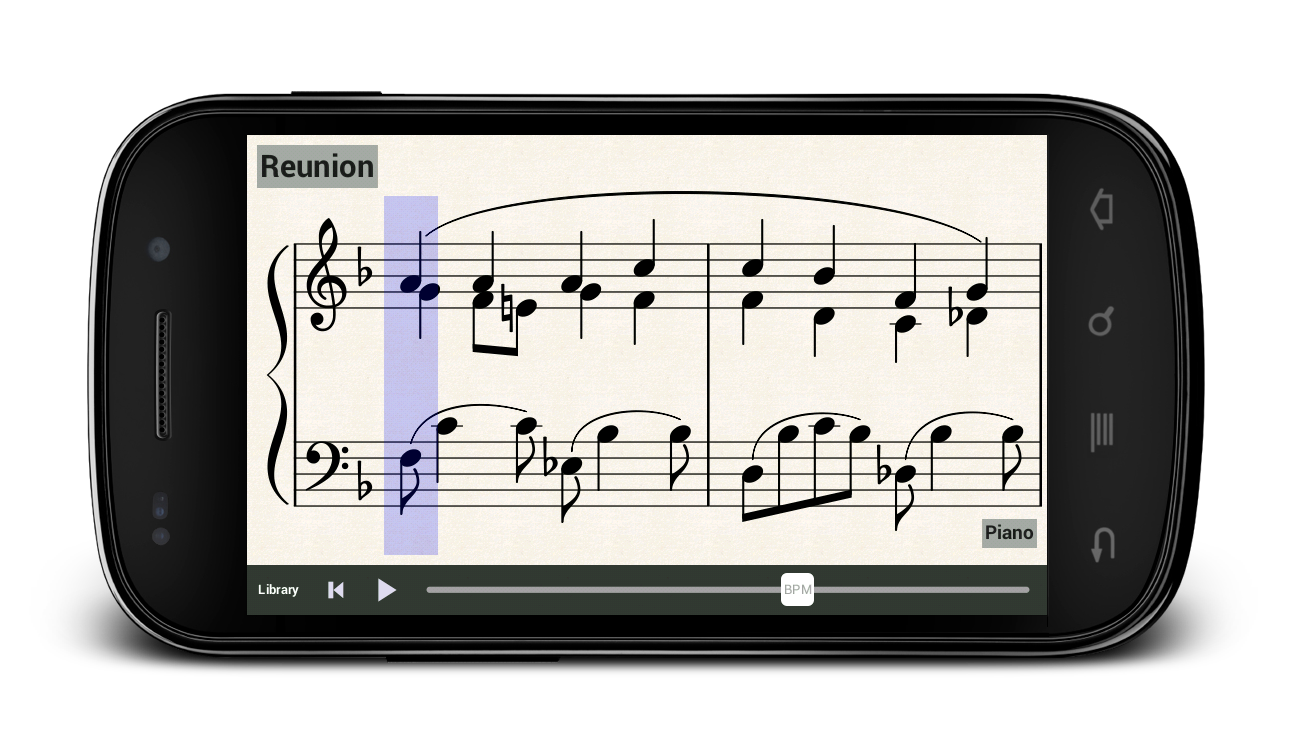
\includegraphics[width=\textwidth]{apps_musescore_android}
\end{frame}

\begin{frame}
  \frametitle{And much more\ldots}
  Autodesk Maya, DAZ Studio, LightWave 3D, Skype, \ldots
  \bigskip

  Find out on \href{https://showroom.qt.io/}{https://showroom.qt.io/}. \pause
  \bigskip

  Now, a small demo of OCaml port.
  \pause
  Well no.

\end{frame}

\begin{frame}
  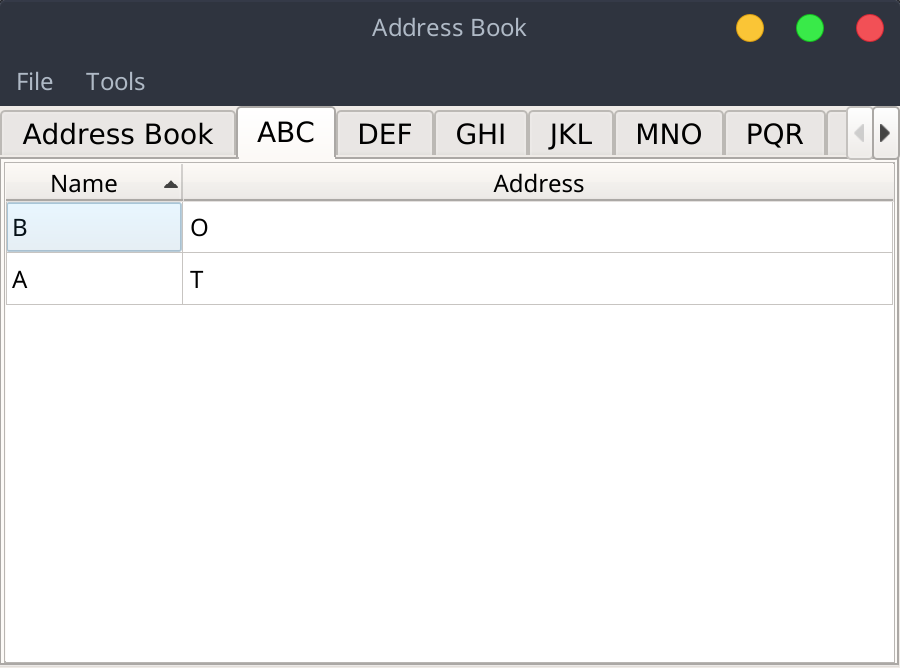
\includegraphics[width=\textwidth]{address_main}
\end{frame}

\begin{frame}
  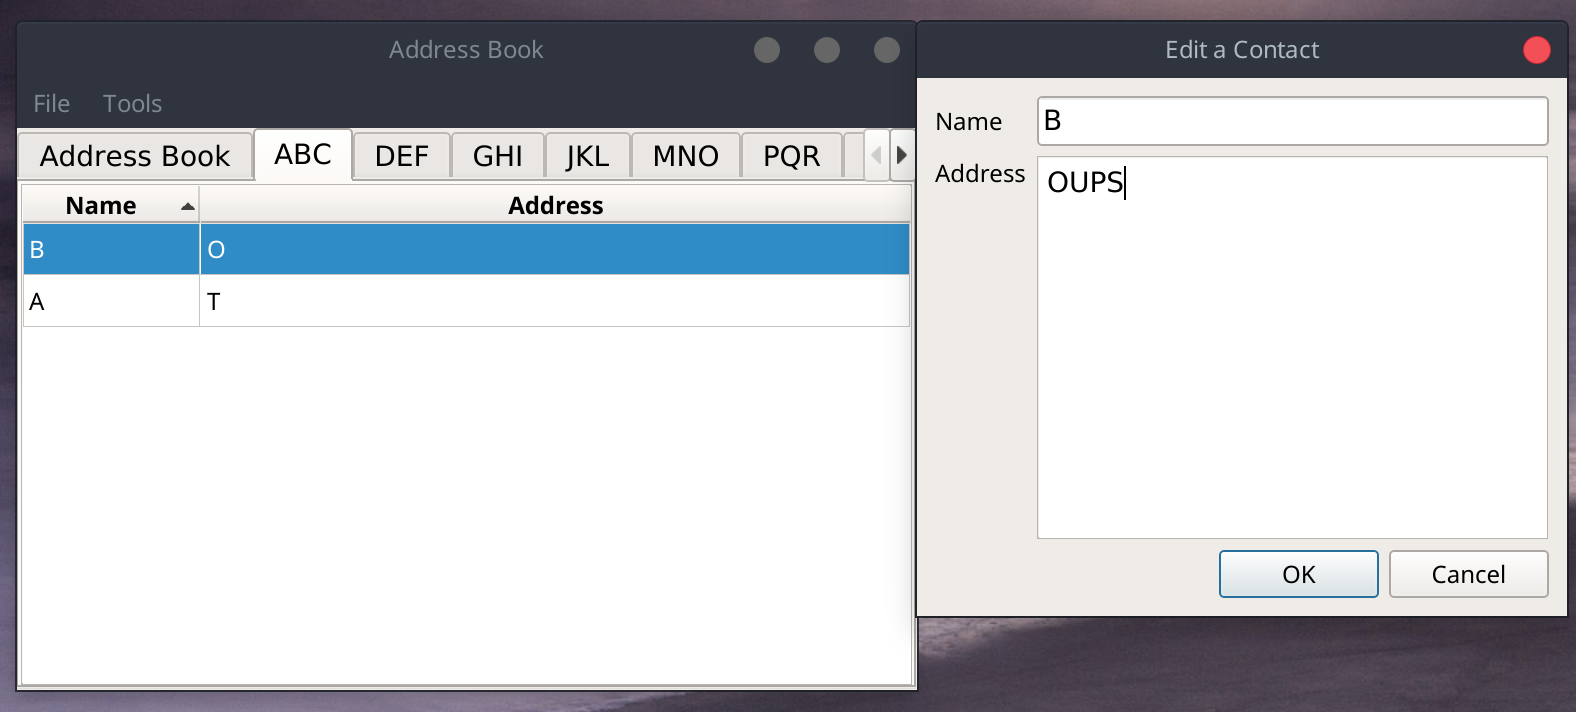
\includegraphics[width=\textwidth]{address_edit}
\end{frame}

\begin{frame}
  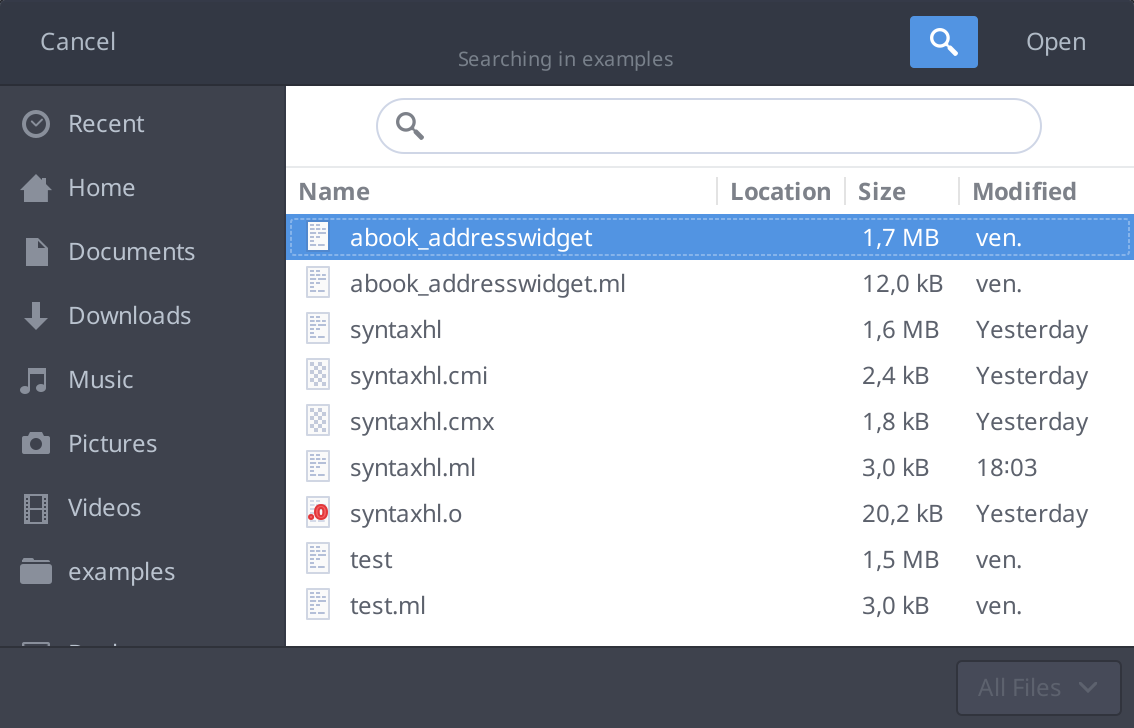
\includegraphics[width=\textwidth]{address_dialog}
\end{frame}

\begin{frame}
  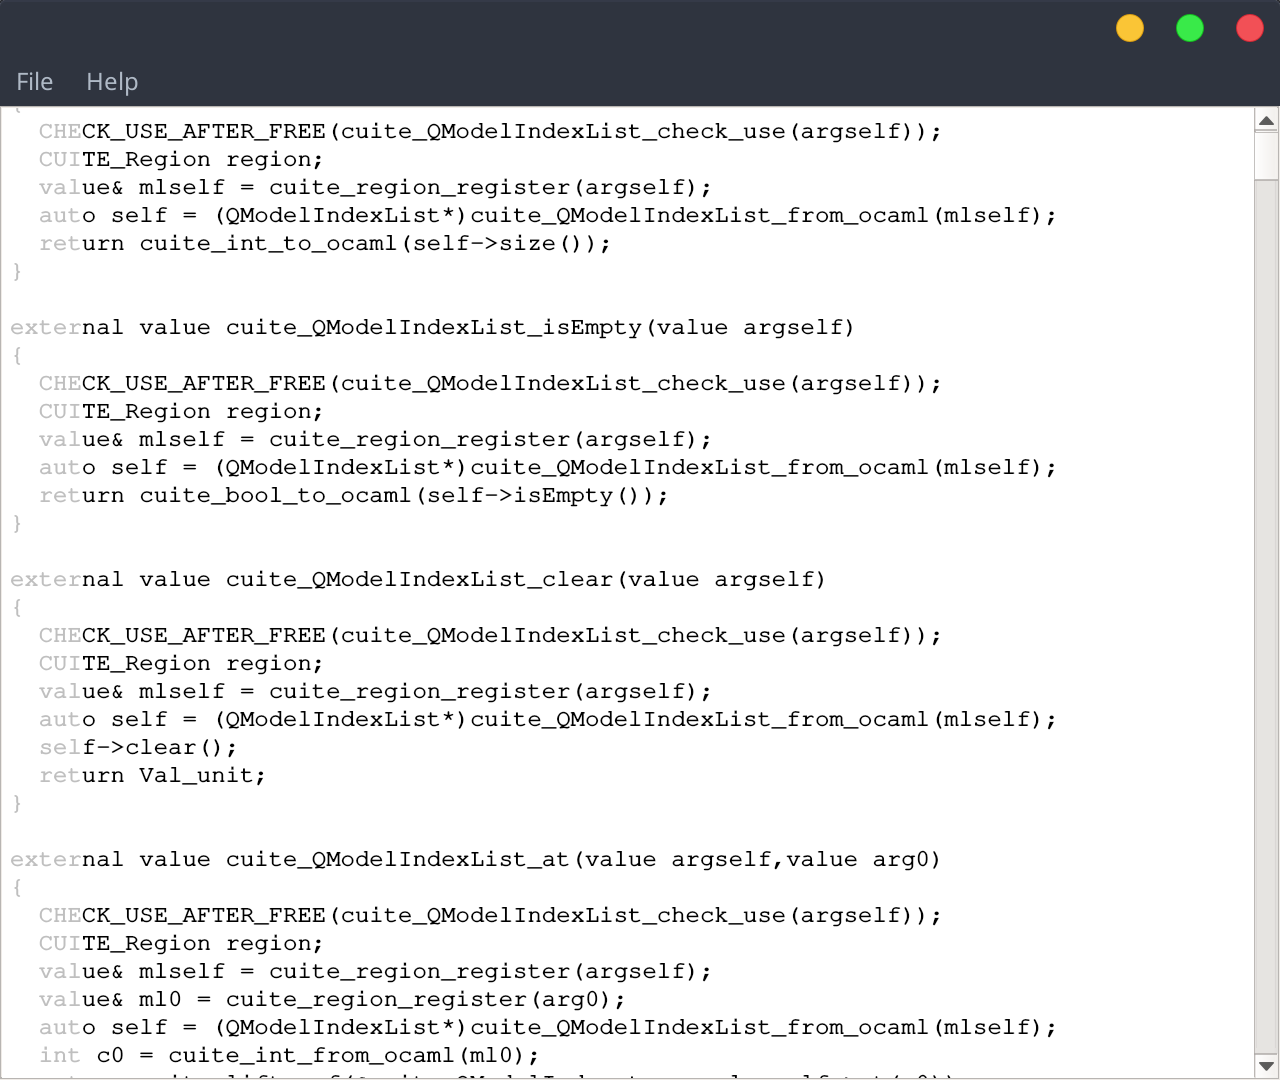
\includegraphics[width=\textwidth]{syntaxhl}
\end{frame}

